\documentclass{boi2014}

\usepackage{enumitem}

\renewcommand{\DayNum}{2}
\renewcommand{\TaskCode}{portals}
\renewcommand{\TaskName}{Portals}
\renewcommand{\TaskVersion}{1.1}

\newcommand{\constant}[1]{{\tt #1}}

\begin{document}
    \begin{wrapfigure}[4]{r}{4cm}
        \vspace{-24pt}
		\includegraphics[width=4cm]{\TaskCode.jpeg}
	\end{wrapfigure}

    There is a cake placed in a labyrinth and you desperately want to eat
    it. You have a map of the labyrinth, which is a grid of $R$ rows and $C$
    columns.  Each grid cell contains one of the following characters:
    \begin{description}[itemindent=1pt]
    	\item[\constant{\#}] (number sign) which denotes a wall block,
        \item[\constant{.}] (dot) which denotes an open square,
        \item[\constant{S}] (uppercase letter s) which denotes an open square of
        your current location,
        \item[\constant{C}] (uppercase letter c) which denotes an open square
        with the cake.
    \end{description}

    You may only walk on the open squares and move from one open square to
    another if they share a side. Additionally, the rectangular area depicted on
    the map is completely surrounded by wall blocks.

    In order to reach the cake faster you have acquired a portal gun from
    Aperture Science\texttrademark{}, which operates as follows.
    At any time it can fire a portal in one of the four directions
    \emph{up}, \emph{left}, \emph{down} and \emph{right}.
    When a portal is fired in some direction, it will fly in that direction
    until it reaches the first wall. When this happens, a portal
    will be spawned on the wall block, on the side that faces you.

    At most two portals can exist at any given time. If two portals are already
    placed in the labyrinth, then one of them (selected by you) will be removed
    immediately upon using the portal gun again. Firing a portal at an existing
    portal will replace it (there may be at
    most one portal per side of wall block).  Note that there may be two portals
    placed on different sides of the same wall block.

    Once two portals are placed in the labyrinth you can use them to
    teleport yourself. When standing next to one of the portals,
    you can walk into it and end up at the open square next to the other
    portal. Doing this takes as much time as moving between two
    adjacent squares.

    You may assume that firing portals does not take time and moving between two
    adjacent squares or teleporting through portals takes one unit of time.

    \Task
    Given the map of the labyrinth together with your starting location
    and the location of the cake, calculate the minimum possible time needed
    for you to reach the cake.

    \Input
    The first line of the input contains two integers: the number of rows
    in the map $R$, and the number of columns $C$. The next $R$ lines describe
    the map. Each of these lines contains $C$ characters: \constant{\#},
    \constant{.}, \constant{S} or \constant{C} (whose meaning is described
    above).

    It is guaranteed that characters \constant{S} and \constant{C} each appear
    exactly once in the map.

    \Output
    The output should contain a single integer --- the minimum time that
    is needed to reach the cake from the starting location.

    You may assume that it is possible to reach the cake from your
    starting location.

    \Example
    \example
    {
        4 4\newline
        .\#.C\newline
        .\#.\#\newline
        ....\newline
        S...
    }
    {
        4
    }
    {
        One quickest sequence of moves is as follows: 1) move right, 2) move
        right, shoot one portal up, and one portal down, 3) move through the
        bottom portal, 4) move one square right and reach the cake.

        \begin{center}
            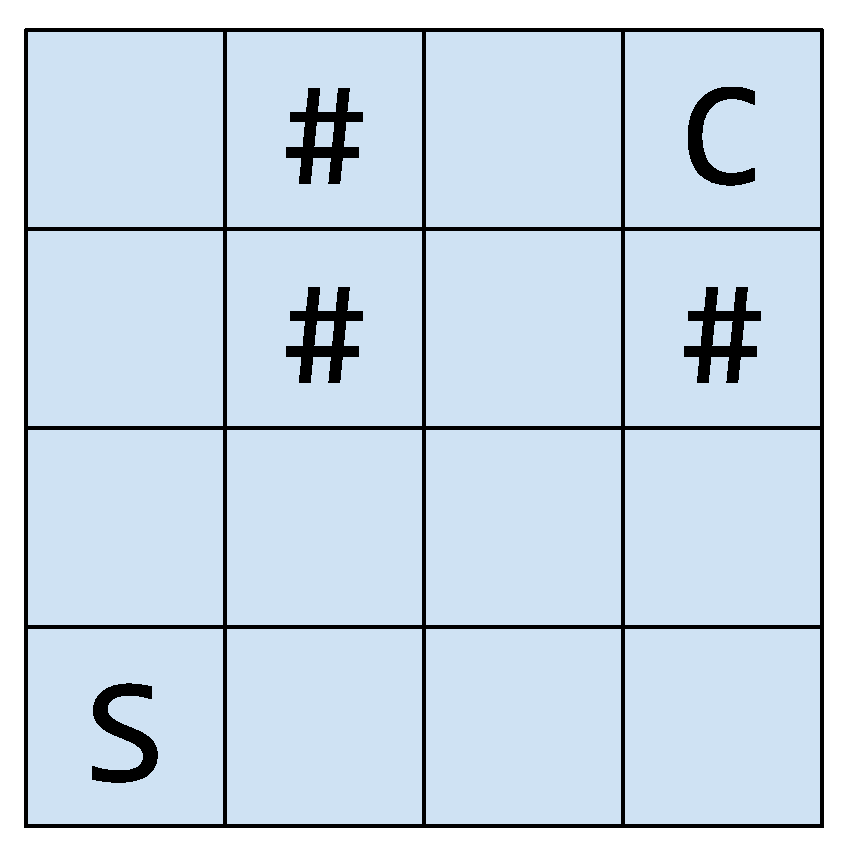
\includegraphics[width=4cm]{portals-example}
        \end{center}
    }

    \Scoring

    \begin{description}[leftmargin=0pt]
        \item[Subtask 1 (11 points):] $1 \le R \le 10, 1 \le C \le 10$.
        \item[Subtask 2 (20 points):] $1 \le R \le 50, 1 \le C \le 50$.
        \item[Subtask 3 (20 points):] $1 \le R \le 200, 1 \le C \le 200$.
        Every open square has at least one wall block adjacent to it.
        \item[Subtask 4 (19 points):] $1 \le R \le 200, 1 \le C \le 200$.
        \item[Subtask 5 (30 points):] $1 \le R \le 1000, 1 \le C \le 1000$.
    \end{description}

    \Constraints

    \begin{description}
        \item[Time limit:] 1 s.
        \item[Memory limit:] 256 MB.
    \end{description}
\end{document}
